In practise arbitrage is the process of buying something at price $x$ and instantly selling it a price $y$ where $x<y$. Arbitrage is risk-free, if we make some assumptions; since we perform it instantly we can gaurentee that $x<y$, and we do not take into account the inherit volunerabilities of bugs in smart contracts.

When determining the arbitrage opportunity it is a bit more complicated since prices of assets are not static but determined by market behaviours. We can see the prices of assets at the different decentralized exchanges, as we defined in the background section there are two main forms of exchanges, the simpler one being the limit order book. When performing arb on LOB DEX's we check if there is some asset (ABC) that has an overlapping price, an example of this can be seen in figure \ref{fig:ArbLOB}, here wee see that we can buy the ABC asset at exchange Y and sell it at exchange X, and we can do that for the overlapping limit orders. 
\begin{figure}[h]
\centering
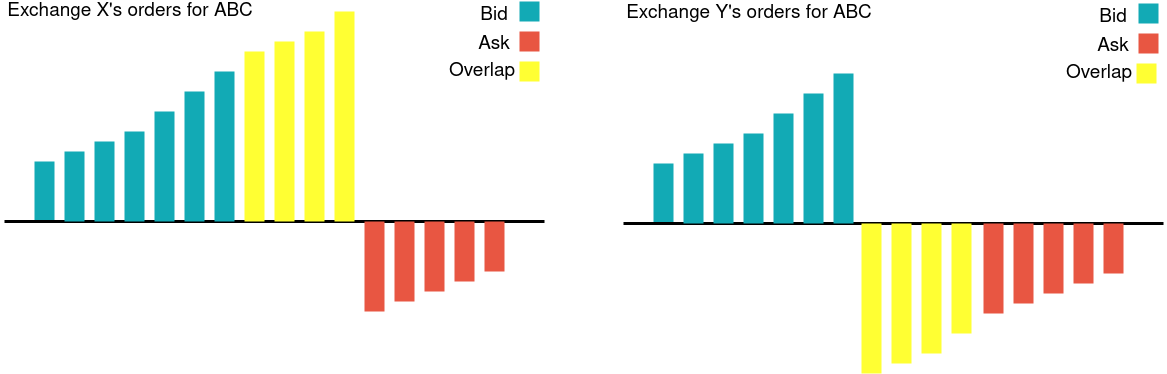
\includegraphics[width=0.7\textwidth]{assests/Flash-loans-Arbitrage-Overlap-1}
\caption{Arbitrage on LOB DEX}
\label{fig:ArbLOB}
\end{figure}
This is a simple form of arbitrage, we can find more opportunities if we look at \textit{triangular arbitrage}. Triangular arbitrage is where the arbitrage opportunity arise from the trade of 3 assets, that is we trade asset X for asset Y, trade asset Y for asset Z, and finally trade asset Z back to asset X. We end up with the rule that if $rate(X/Y)*rate(X/Z)>rate(Y/X)$ then there is a profitable arbitrage (where $rate(A/B)$ is the conversion rate from $B$ to $A$). We have visualized this with an example in figure \ref{ArbTrig}.
\begin{figure}[h]
\centering
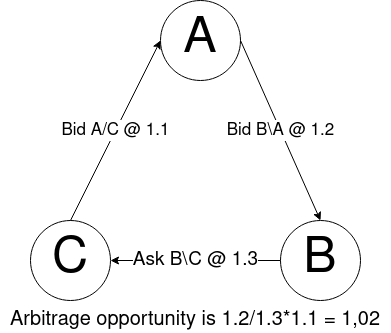
\includegraphics[width=0.4\textwidth]{assests/Flash-loans-Arbitrage-triangular}
\caption{Triangular arbitrage}
\label{fig:ArbTrig}
\end{figure}